\documentclass[12pt]{article}
\usepackage[spanish,mexico]{babel}
	\selectlanguage{spanish}
\usepackage{graphicx}
\usepackage{amsmath}
\usepackage{wrapfig}
\usepackage{float}
\usepackage[utf8]{inputenc}

\usepackage{graphicx}
\graphicspath{{images/}}

\usepackage{vmargin}
\setmarginsrb{3 cm}{1.0 cm}{3 cm}{1.0 cm}{1 cm}{1.5 cm}{1 cm}{1.5 cm}
\usepackage{listings}
\usepackage[usenames,dvipsnames]{color}
	\definecolor{ocre}{RGB}{42,105,21}
	\definecolor{ocre2}{RGB}{47,109,130}
	\definecolor{gray2}{gray}{0.95}
	\lstset{
		language=Python,
		backgroundcolor=\color{gray2},
		basicstyle=\color{black}\small\ttfamily, 
		breakatwhitespace=false,         
		breaklines=true,                 
		captionpos=b,                    
		columns=flexible,
		commentstyle=\color{ocre2}\ttfamily, 
		deletekeywords={...},            
		escapeinside={\%*}{*)},          
		extendedchars=true,             
		frame=single,	                 
		keepspaces=true,                 
		keywordstyle=\color{blue}\bfseries,       
		otherkeywords={*,...},          
		numbers=left,                    
		numbersep=5pt,                   
		numberstyle=\tiny, 
		rulecolor=\color{black},         
		showspaces=false,                
		showstringspaces=false,          
		showtabs=false,                  
		stepnumber=1,                    
		stringstyle=\normalfont\color{ocre},     
		tabsize=2,	                     
		title=\lstname                  
		}

\title{Actividad 5: Movimiento armónico simple:\\ Péndulo}
\author{Martin Alejandro Paredes Sosa}
\date{Marzo, 2016}

\begin{document}
\maketitle

\section{Introducción}
Un espacio fase es una representación geométrica de las trayectorias de un sistema dinámico en el plano fase. Cada set de condiciones iniciales esta representada por una curva o punto. Este es una herramienta muy útil en el estudio de los sistemas dinámicos.

En el espacio fase, cada grado de libertad o parámetro del sistema se representa por un eje coordenado en el espacio multidimensional. Un sistema con dos parámetros suele ocurrir para una sola partícula moviéndose en una dimensión, donde las variables son posición y velocidad.

La ecuación diferencial que representa el movimiento del péndulo simple es:
\begin{equation}\label{Pen}
	\frac{d^2\theta}{dt^2}+\frac{g}{\ell}\sin\theta=0
\end{equation}
donde $g$ es la aceleración debida a la gravedad, $\ell$ la longitud del péndulo y $\theta$ es el desplazamiento angular.


\section{Función \emph{integrate.odeint}}
La ecuación diferencial del péndulo no tiene una solución analítica. Para poder resolverla se utilizan herramientas computacionales. En nuestro caso, para resolverla se utiliza la función \emph{integrate.odeint} de la librería \emph{scipy} de Python \cite{scipy}.

Esta función utiliza los siguientes parámetros:
\begin{itemize}
	\item func: \textit{callable(y, t0, ...)}. Computa la derivada de y en t0.
	\item y0: \textit{arreglo}. Las condiciones iniciales en y. Puede ser un vector.
	\item t:\textit{arreglo}. Secuencia de puntos para los cuales se resolverá y. El valor inicial debe ser el primer valor se la secuencia.
	\item args:\textit{tuple, opcional}. Argumentos extra para la función.
\end{itemize}

\section{Ejercicio y Resultados}
Esta actividad consistió en realizar un código en python que nos permitiera construir el espacio fase de un péndulo simple. Se hizo uso de la librería \emph{scipy.integrate} haciendo uso de la función \textit{odeint} para resolver la ecuacion \eqref{Pen} y asi conocer todas las trayectorias. \\

El código que se utilizo fue el siguiente:
\lstinputlisting[caption={Programa Fase.py}]{Fase.py}

El resultado que se obtuvo fue el siguiente:
\begin{figure}[H]
\centering
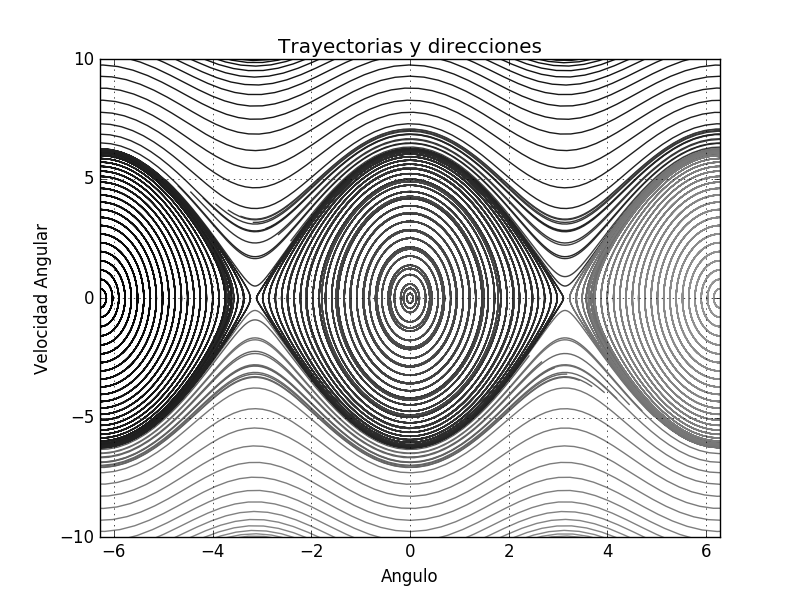
\includegraphics[width=15cm, height=8.5cm]{DFase.png}
\caption{Diagrama Fase del péndulo simple}
\end{figure}

%============================================================================================================
\pagebreak

\begin{thebibliography}{4}

	\bibitem{PendWiki}
	Wikipedia,(2015)
	\emph{Phase portrait}. Recuperado de\\
	https://en.wikipedia.org/wiki/Phase\_portrait

	\bibitem{scipy}
	Scipy.org (2016)
	\emph{Integration and ODEs}. Recuperado de\\
	http://docs.scipy.org/doc/scipy/reference/generated/scipy.integrate.odeint.html\\\#scipy.integrate.odeint

	\bibitem{act}
	Lizárraga, C. (2016)
	\emph{Actividad 7 (2016-1)}. Recuperado de\\ 
	http://computacional1.pbworks.com/w/page/105676740/Actividad\%207\%20\\(2016-1)
	
	\bibitem{cookbook}
	Scipy Cookbook (2015)
	\emph{Matplotlib: lotka volterra tutorial}. Recuperado de:\\
	http://scipy-cookbook.readthedocs.org/items/LoktaVolterraTutorial.html	
		
\end{thebibliography}
\end{document}